\documentclass[a4paper]{article}

\usepackage[utf8]{inputenc}
\usepackage[T1]{fontenc}
\usepackage{textcomp}
\usepackage[english]{babel}
\usepackage{amsmath, amssymb}


%figure support
\usepackage{import}
\usepackage{xifthen}
\pdfminorversion=7
\usepackage{pdfpages}
\usepackage{transparent}
\newcommand{\incfig}[1]{%
	\def\svgwidth{\columnwidth}
	\import{./figures/}{#1.pdf_tex}
}

\graphicspath{ {figures/} }

\pdfsuppresswarningpagegroup=1

\begin{document}
	\title{CAP4630.01 Assignment 3: Due 10/3/2019}
	\author{Brandon Thompson 5517}
	\maketitle
	\medskip
	Given the following search tree, state the order in which the nodes will be visited by
	using \textbf{hill climbing, steepest ascent hill climbing, depth-first iterative
	deepening} and \textbf{beam search with width $= 3$}. The numbers on the nodes indicate
	the estimated cost to the goal.

	\begin{figure}[ht!]
		\centering
		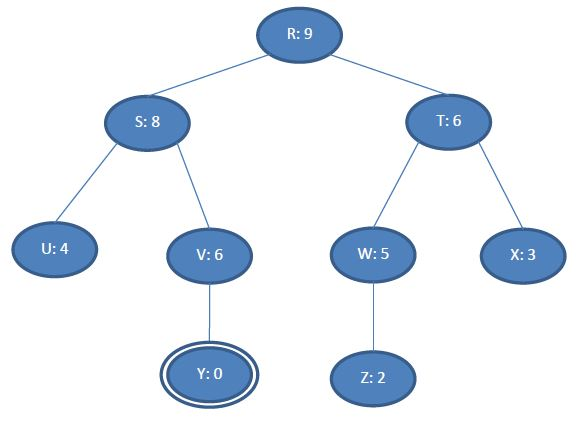
\includegraphics[width=0.8\textwidth]{SearchTree}
		\caption{Search tree}
		\label{fig:st}
	\end{figure}
	\begin{description}
		\item[Hill climbing:] R:9, S:8, U:4.\\
			R has distance of 9, first child of R with lower distance is S:8.\\
			First child of S with lower distance is U:4.\\
			U has no children, goal node not found.
		\item[Steepest ascent hill climbing:] R:9, T:6, X:3.\\
			Same as \textbf{Hill climbing} except that it will always take the best of the child nodes
			no matter the node expansion. Goal node not reached.
		\pagebreak
		\item[Depth-first iterative deepening:] R:9, R:9, S:8, T:6, R:9, S:8, U:4, V:6, T:6, W:5, X:,3
			R:9, S:8, U:4, V:6, Y:0.\\
			Do depth-limited search for depths $=0 \to 3$ until goal node is reached.\\
			DLS depth $=0$: R\\
			DLS depth $=1$: R, S, T\\
			DLS depth  $=2$: R, S, U, V, T, W, X\\
			DLS depth  $=3$ : R, S, U, V, Y
		\item[Beam search, width = 3:] R:9, T:6, X:3, W:5, Z:2, S:8, U:4, V:6, Y:0.\\
			Search node R, add children to queue and sort, T:6, S:8.\\
			Search T:6, add children to queue, X:3, W:5, S:8 search X:3, no goal state.\\
			Search W:5, add children to queue, Z:2, S:8, search Z:2, no goal state.\\
			Search S:8, add children to queue, U:4, V:6, search U:4, no goal state.\\
			Search V:6, add children to queue, Y:0, search Y:0, goal state found.
	\end{description}
\end{document}
